\documentclass[tikz,border=2pt]{standalone}
\usepackage{amsmath,amssymb}
\usepackage{pgfplots}
\pgfplotsset{compat=1.18}
\usetikzlibrary{calc}

\begin{document}
% X ~ U(0,1) and Y = X^2: the flat density of X is squeezed near 0 (where g is flat) and
% stretched near 1, giving f_Y(y) = 1/(2 sqrt y) via the change-of-variables formula.
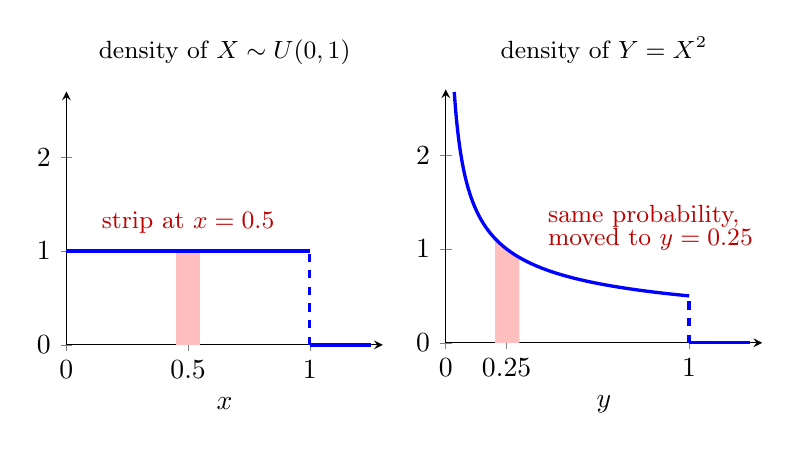
\begin{tikzpicture}
	\begin{axis}[
		name=p1, axis lines=left, xmin=0, xmax=1.3, ymin=0, ymax=2.7,
		xtick={0,0.5,1}, ytick={0,1,2},
		xlabel={$x$},
		width=5.6cm, height=4.8cm, clip=false, title={density of $X\sim U(0,1)$}, title style={font=\small}
		]
		\fill[red!25] (axis cs:0.45,0) rectangle (axis cs:0.55,1);
		\draw[blue, very thick] (axis cs:0,1) -- (axis cs:1,1);
		\draw[blue, very thick, dashed] (axis cs:1,0) -- (axis cs:1,1);
		\draw[blue, very thick] (axis cs:1,0) -- (axis cs:1.25,0);
		\node[red!75!black, font=\small, anchor=south] at (axis cs:0.5,1.08) {strip at $x=0.5$};
	\end{axis}
	\begin{axis}[
		name=p2, at={(p1.outer east)}, anchor=outer west, xshift=3mm,
		axis lines=left, xmin=0, xmax=1.3, ymin=0, ymax=2.7,
		xtick={0,0.25,1}, xticklabels={$0$,$0.25$,$1$}, ytick={0,1,2},
		xlabel={$y$},
		samples=200, smooth, width=5.6cm, height=4.8cm, clip=false, title={density of $Y=X^2$}, title style={font=\small}
		]
		\fill[red!25] (axis cs:0.2025,0) -- (axis cs:0.2025,1.111) -- (axis cs:0.3025,0.909) -- (axis cs:0.3025,0) -- cycle;
		\addplot[blue, very thick, domain=0.035:1] {1/(2*sqrt(x))};
		\draw[blue, very thick, dashed] (axis cs:1,0) -- (axis cs:1,0.5);
		\draw[blue, very thick] (axis cs:1,0) -- (axis cs:1.25,0);
		\node[red!75!black, font=\small, anchor=west] at (axis cs:0.38,1.35) {same probability,};
		\node[red!75!black, font=\small, anchor=west] at (axis cs:0.38,1.1) {moved to $y=0.25$};
	\end{axis}
	
\end{tikzpicture}
\end{document}
